\documentclass[11pt]{article}

% Paquetes
%===================================================================================================

% Paquete para incluir codigo
\usepackage{listings}

% Paquete para incluir imagenes
\usepackage{graphicx}
\graphicspath{ {./Imagenes/} }

% Para que el codigo acepte caracteres en utf8
\lstset{literate=
  {á}{{\'a}}1 {é}{{\'e}}1 {í}{{\'i}}1 {ó}{{\'o}}1 {ú}{{\'u}}1
  {Á}{{\'A}}1 {É}{{\'E}}1 {Í}{{\'I}}1 {Ó}{{\'O}}1 {Ú}{{\'U}}1
  {à}{{\`a}}1 {è}{{\`e}}1 {ì}{{\`i}}1 {ò}{{\`o}}1 {ù}{{\`u}}1
  {À}{{\`A}}1 {È}{{\'E}}1 {Ì}{{\`I}}1 {Ò}{{\`O}}1 {Ù}{{\`U}}1
  {ä}{{\"a}}1 {ë}{{\"e}}1 {ï}{{\"i}}1 {ö}{{\"o}}1 {ü}{{\"u}}1
  {Ä}{{\"A}}1 {Ë}{{\"E}}1 {Ï}{{\"I}}1 {Ö}{{\"O}}1 {Ü}{{\"U}}1
  {â}{{\^a}}1 {ê}{{\^e}}1 {î}{{\^i}}1 {ô}{{\^o}}1 {û}{{\^u}}1
  {Â}{{\^A}}1 {Ê}{{\^E}}1 {Î}{{\^I}}1 {Ô}{{\^O}}1 {Û}{{\^U}}1
  {ã}{{\~a}}1 {ẽ}{{\~e}}1 {ĩ}{{\~i}}1 {õ}{{\~o}}1 {ũ}{{\~u}}1
  {Ã}{{\~A}}1 {Ẽ}{{\~E}}1 {Ĩ}{{\~I}}1 {Õ}{{\~O}}1 {Ũ}{{\~U}}1
  {œ}{{\oe}}1 {Œ}{{\OE}}1 {æ}{{\ae}}1 {Æ}{{\AE}}1 {ß}{{\ss}}1
  {ű}{{\H{u}}}1 {Ű}{{\H{U}}}1 {ő}{{\H{o}}}1 {Ő}{{\H{O}}}1
  {ç}{{\c c}}1 {Ç}{{\c C}}1 {ø}{{\o}}1 {å}{{\r a}}1 {Å}{{\r A}}1
  {€}{{\euro}}1 {£}{{\pounds}}1 {«}{{\guillemotleft}}1
  {»}{{\guillemotright}}1 {ñ}{{\~n}}1 {Ñ}{{\~N}}1 {¿}{{?`}}1 {¡}{{!`}}1
}

% Para que los metadatos que escribe latex esten en español
\usepackage[spanish]{babel}

% Para la bibliografia
% Sin esto, los enlaces de la bibliografia dan un error de compilacion
\usepackage{url}

% Metadatos del documento
%===================================================================================================
\title{
    {Aprendizaje Automático - Segunda Práctica}\\
    {Complejidad de $H$ y el ruido}\\
    {Modelos Lineales}
}

\author{
    {Sergio Quijano Rey - 72103503k}\\
    {4º Doble Grado Ingeniería Informática y Matemáticas}\\
    {sergioquijano@correo.ugr.es}
}

\date{\today}

% Separacion entre parrafos
\setlength{\parskip}{1em}


% Contenido del documento
%===================================================================================================
\begin{document}

% Portada del documento
\maketitle
\pagebreak

% Indice de contenidos
\tableofcontents
\pagebreak

\section{Ejercicio 1 - Sobre la complejidad de $H$ el ruido}

\subsection{Observaciones iniciales}

Para este primer ejercicio, hacemos uso de tres funciones que se nos dan en el fichero \lstinline{template_trabajo2.py}. Las dos primeras funciones devuelven una lista de $N$ vectores de una dimensión dada.

\begin{itemize}
    \item \lstinline{simula_unif}: genera una lista de $N$ vectores aleatorios de una dimensión dada. La distribución aleatoria que siguen es una distribución uniforme en un intervalo dado
    \item \lstinline{simula_gauss}: genera una lista de $N$ vectores aleatorios de dimensión dada. La distribución aleatoria es una normal de media cero y varianza dada
    \item \lstinline{simula_recta}: genera una recta aleatoria que pasa a través de un intervalo 2-dimensional dado
\end{itemize}

Además, al principio de cada función asociada a los ejercicios (\lstinline{ejercicio1()}, \lstinline{ejercicio2()}, \lstinline{ejercicio_bonus()}) establecemos una semilla aleatoria fija con la orden \lstinline{np.random.seed(123456789)}. Así, los resultados que obtenemos serán reproducibles. Aunque por estar usando probablemente distintos configuraciones de sistemas operativos, hardware, versión de \lstinline{python}, \ldots, los resultados obtenidos por los profesores de prácticas no serán exactamente los mismos cuando exista un factor aleatorio.

\subsection{Apartado 1}

En este apartado se pide que dibujemos las nubes de puntos simuladas con las dos primeras funciones dadas por los profesores. Para ello empleamos los siguientes parámetros:

\begin{itemize}
    \item $N = 50$
    \item $dim = 2$
    \item $rango = [-50, 50]$
    \item $\sigma = [5, 7]$ donde $\sigma$ indica la varianza (por tanto sería más adecuada la notación $\sigma^2$) en el eje $x$ e $y$
\end{itemize}

Lanzando el código obtenemos las dos siguientes nubes de puntos:

\begin{figure}[h]
    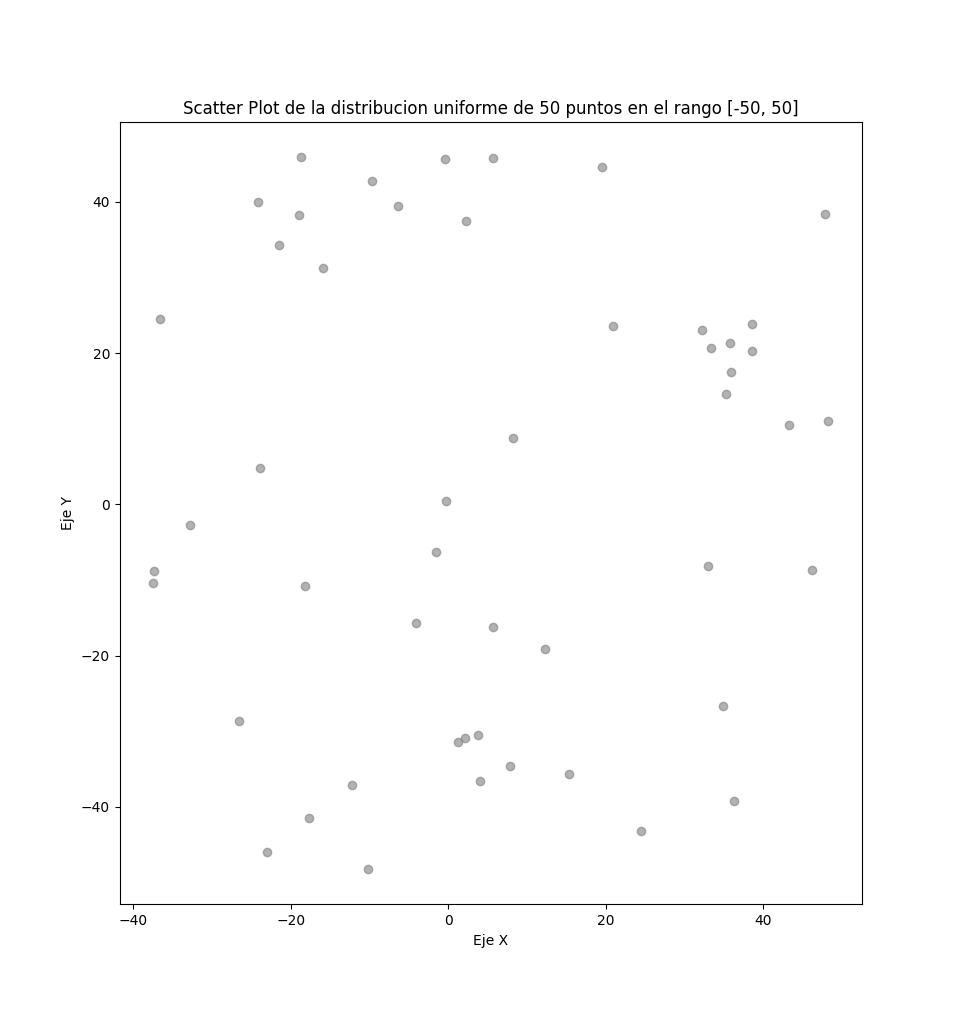
\includegraphics[width=0.60 \textwidth]{nube_puntos_uniforme}
    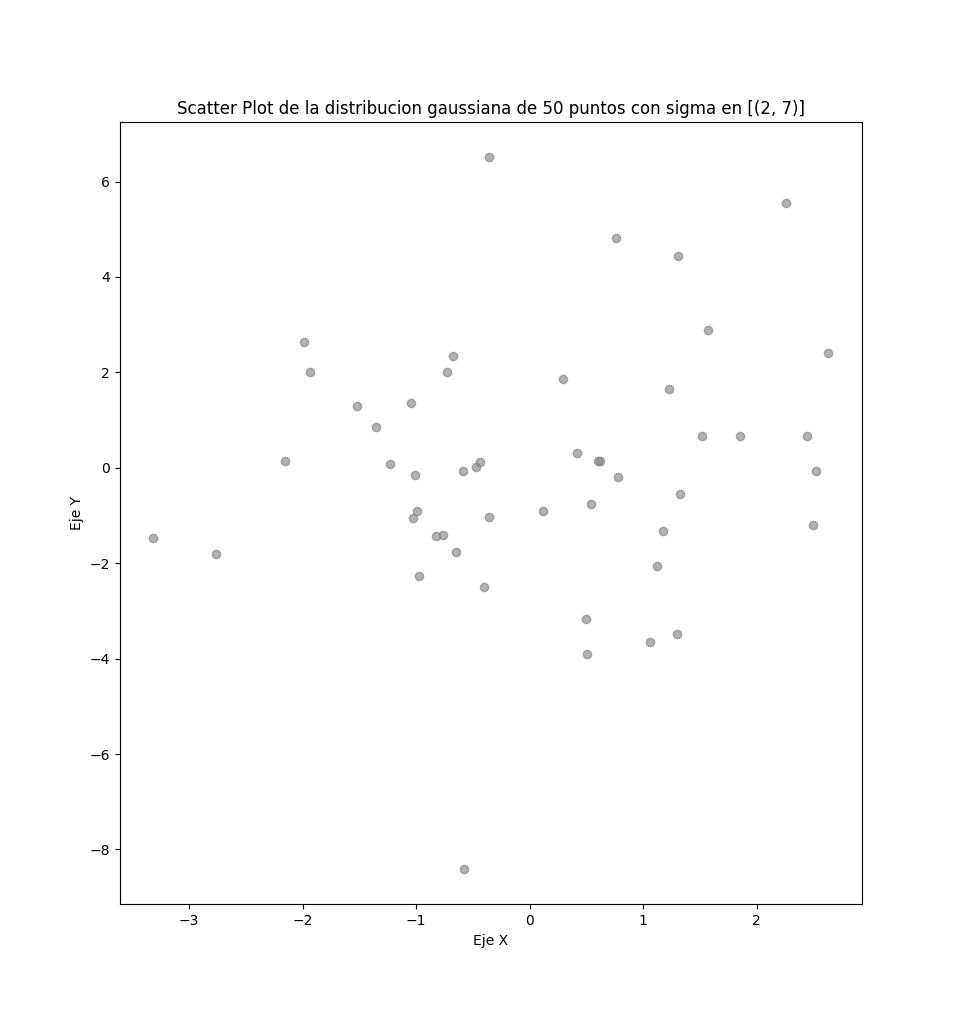
\includegraphics[width=0.60 \textwidth]{nube_puntos_normal}
    \caption{Nubes de puntos de las dos distribuciones}
\end{figure}

\subsection{Apartado 2}

Vamos a valorar la influencia del ruido en la selección dela complejidad de la clase de funciones. Para ello generamos una muestra de puntos bidimensionales. En concreto, generamos 100 puntos en el intervalo $[-50, 50]$.

Una vez que generamos esta muestra de datos, los etiquetamos usando una recta generada aleatoriamente, usando la función dada por los profesores \lstinline{simula_recta}. Con la recta $f(x) = ax + b$, etiquetamos los datos con la función de etiquetado $(x, y) \rightarrow sign(y - ax - b)$. Esta función toma un punto $x, y$, calcula su distancia a la recta $f$ (que se corresponde con $y - f(x)$) y como etiqueta asigna el signo de esta distancia. Es decir, estamos mirando si un punto se queda por encima de la recta (etiqueta $+1$) o por debajo (etiqueta $-1$).

\subsubsection{Subapartado a)}

El enunciado de este apartado especifica que se vuelva a generar la muestra de datos, como se especifica anteriormente. Por tanto, se puede ver que la nube de datos no es la misma que la nube de datos uniforme del Apartado 1.

La gráfica de los datos etiquetados, junto a la recta que se usa para etiquetar, es la siguiente:

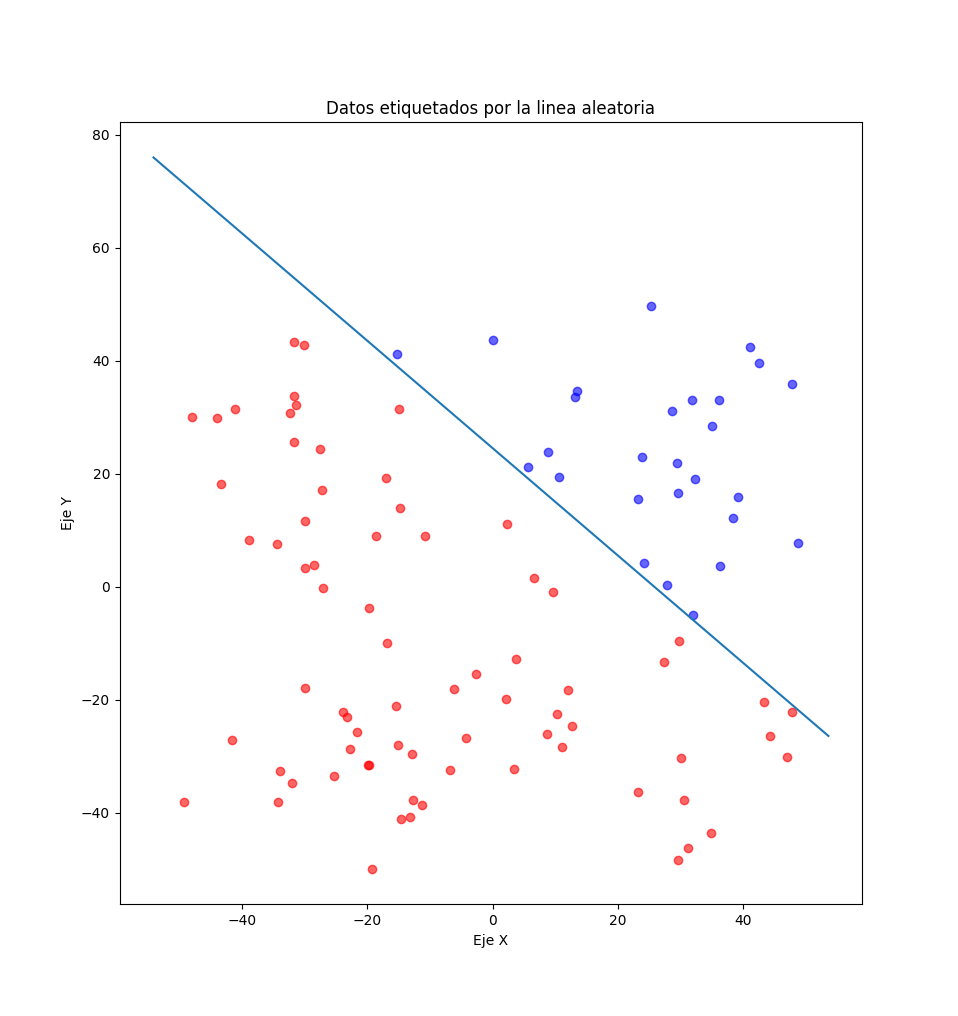
\includegraphics[width=0.9 \textwidth]{puntos_clasificados_recta01}

La gráfica deja claro que los puntos han sido correctamente clasificados a partir de la recta generada aleatoriamente.

\subsubsection{Subapartado b)}

Modificamos el 10\% de las etiquetas positivas y un 10\% de las etiquetas negativas, y volvemos a mostrar la gráfica.

Para realizar esto de forma eficiente, lo que hacemos es tomar dos vectores, uno con las posiciones de etiquetas positivas y otro con las posiciones de las etiquetas negativas. Calculamos el número de etiquetas de cada tipo a cambiar ($N_1, N_2$), a partir de un porcentaje arbitrario (para nuestro caso concreto, usamos $0.1$). Hacemos un \emph{shuffle} de los dos vectores de posiciones y cambiamos el etiquetado de las $N_1$ y $N_2$ primeras posiciones del vector remezclado. Con ello modificamos un porcentaje dado de las etiquetas de forma aleatoria. Todo esto se puede ver en la función \lstinline{change_labels}.

Notar que podemos tener clases sin puntos. Es decir, que no etiquetamos ningún dato con o bien $+1$ o bien $-1$. En el caso de la recta, es muy improbable que esto pase. Pero en el siguiente subapartado, con ciertas funciones es muy probable que pase.

El gráfico de clasificación tras esta modificación aleatoria es:

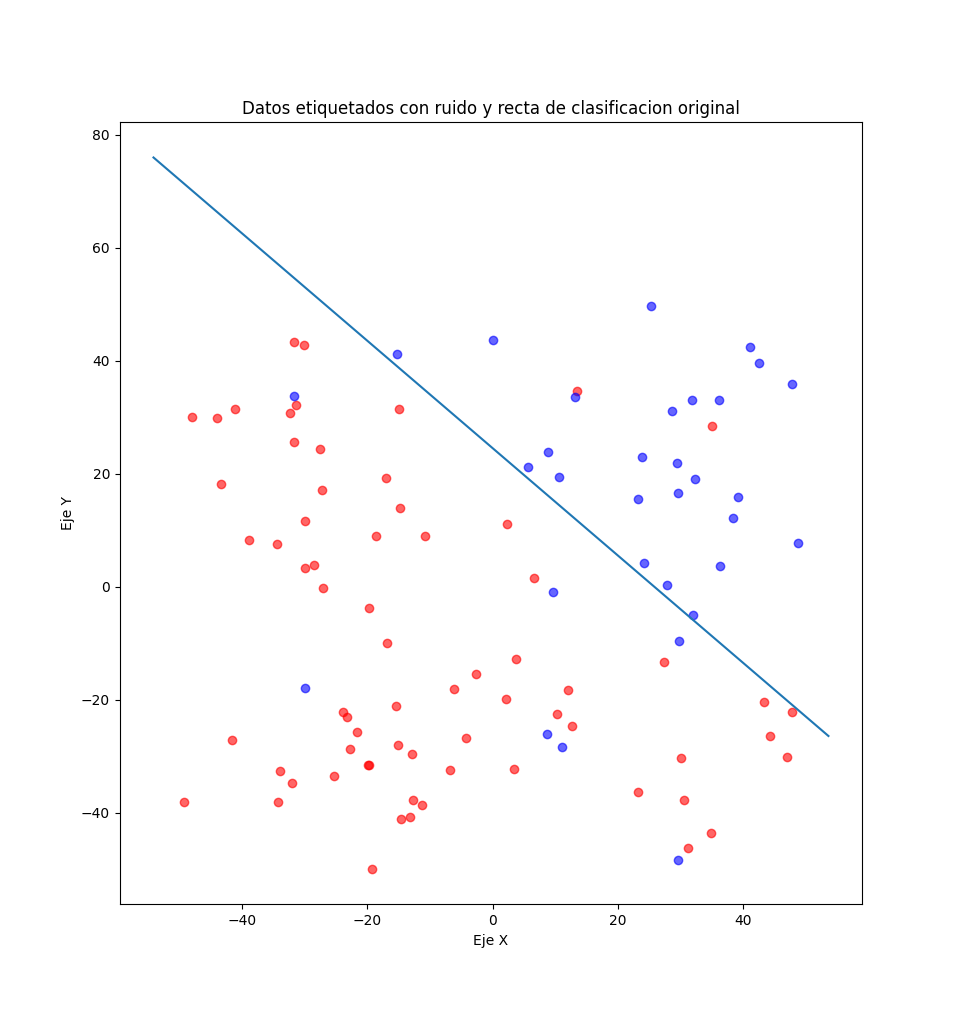
\includegraphics[width = 0.8 \textwidth]{puntos_clasificados_recta_aleatorizados01}

Se ve con claridad cómo esta operación introduce ruido sobre nuestras etiquetas.

\subsubsection{Subapartado c)}

Consideramos ahora las siguientes funciones que definen una frontera de clasificación:

\begin{itemize}
    \item $f_1(x, y):= (x - 10)^2 + (y - 20)^2 - 400$
    \item $f_2(x, y):= \frac{1}{2} (x + 10)^2 + (y - 20)^2 - 400$
    \item $f_3(x, y):= \frac{1}{2} (x - 10)^2 - (y + 20)^2 - 400$
    \item $f_4(x, y):= y - 20x^2 -5x +3$
\end{itemize}

Usamos estas funciones de frontera para clasificar los datos generados en el Subapartado a). También modificamos un 10\% de las etiquetas positivas y negativas aleatoriamente. Además, mostramos las regiones de clasificado positivo y negativo de las funciones empleadas.

% TODO -- comente si estas funciones mas complejas son mejores clasificadores que la funcion lineal
% TODO -- observe las graficas y diga que consecuencias extrae sobre la influencia del proceso de modificacion de etiquetas en el proceso de aprendizaje
% TODO -- para esto ultimo decir que no tiene demasiado sentido. Cambiamos el valor de las etiquetas del 10% de los datos, independientemente de las caracteristicas de la función. Otra discusión seria posible si modificasemos las coordeandas de un punto, en cuyo caso si podemos considerar la tolerancia del clasificador frente al ruido. Esta forma sintética de introducir ruido no nos permite realizar consideraciones sobre lo buenas que son las funciones


% Bibliografia
\bibliography{References}
\bibliographystyle{ieeetr}

\end{document}
